\section{Metaheuristiken} \label{sec:Metaheuristiken}
Optimierungsprobleme lassen sich im Grundlegenden in zwei Kategorien klassifizieren, nämlich in diskrete und kontinuierliche Optimierungsprobleme. Bei dem diskreten Fall existiert zur Lösungsfindung kein Wissen über einen exakten polynomialen Algorithmus und somit handelt es sich hierbei um ein NP-hartes Problem. Beim kontinuierlichen Fall existiert kein Wissen über einen Algorithmus zur Findung des globalen Optimums, welche die bestmögliche Lösung innerhalb eines endlichen Lösungsraums darstellt. \cite[vgl.][S. 2]{siarry_metaheuristics_2016}\\

Heuristiken können in diskreten Optimierungsproblemen eingesetzt werden, um passable Lösungen zu identifizieren, z. B. über Aktivititätsregeln beim \ac{rcpsp} (vgl. Abschnitt \ref{subsec:SGS_Aktivitaeten}). Diese Heuristiken sind dennoch kein Garant für das Finden vom globalen Optimum. Zudem sind Heuristiken für jeweils ein konkretes Problem entwickelt worden und können nicht auf andere Optimierungsprobleme angewandt werden \cite[vgl.][S. 2]{siarry_metaheuristics_2016}. \\


\begin{figure}[H]
    \centering
    \noindent\makebox[\textwidth]{%
    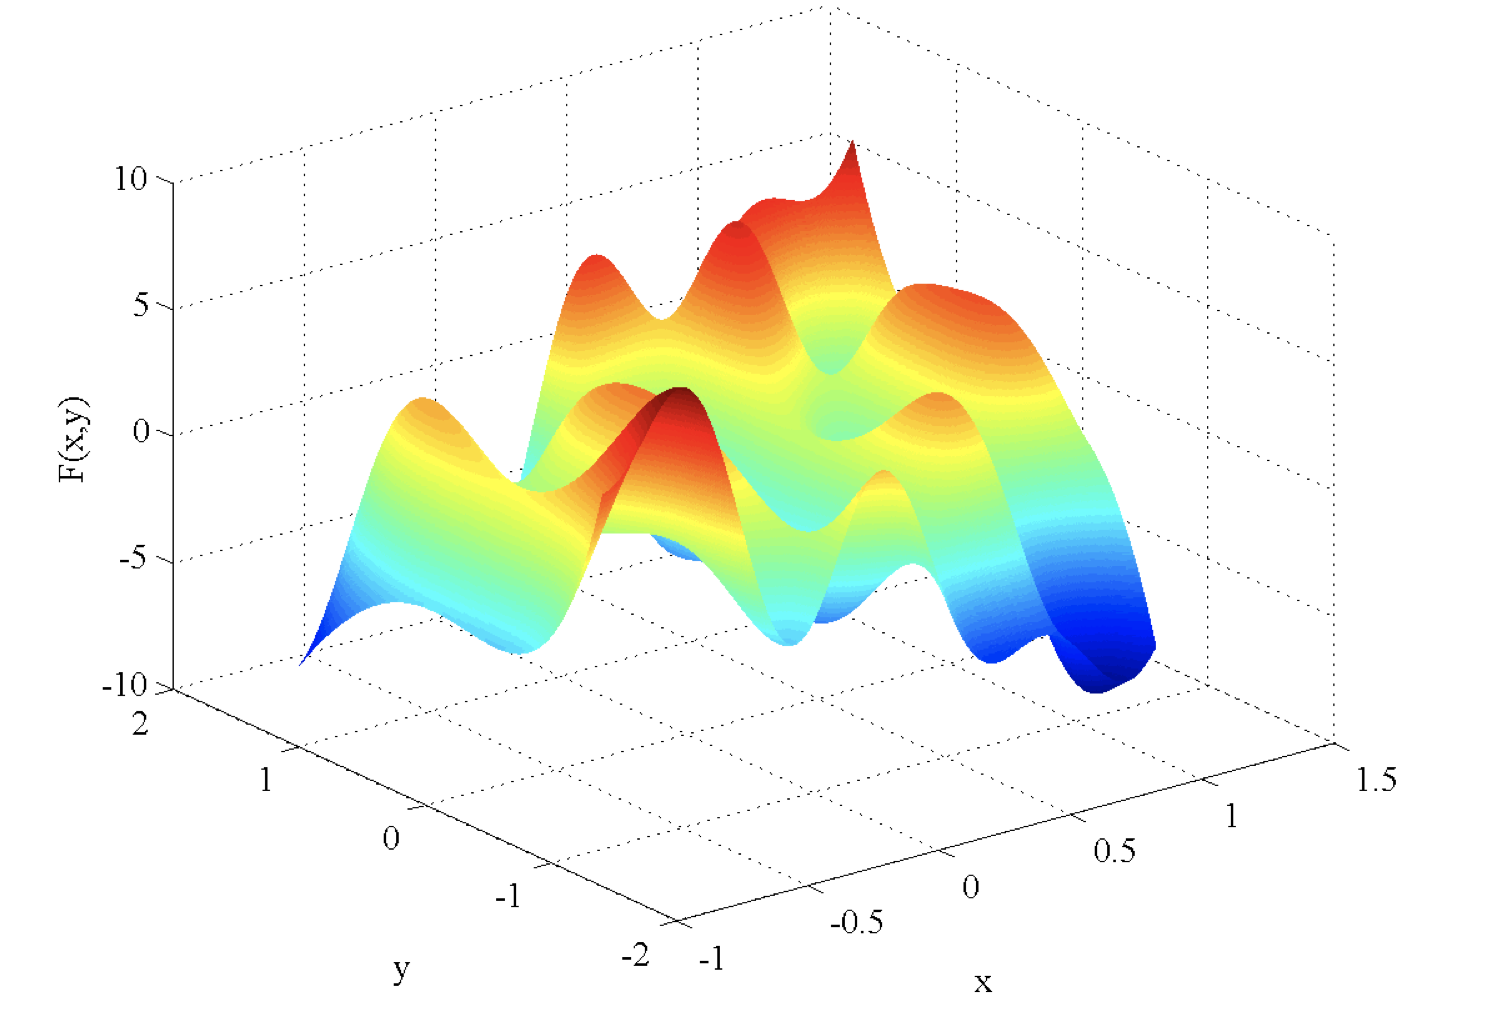
\includegraphics[width=0.9\textwidth]{assets/img/02_Grundlagen/ExampleSearchspace.png}
    }
    \caption{Beispielhafte Darstellung eines kontinuierlichen Such- oder Optimierungsraums einer Zielfunktion $f(x, y)$ mit zwei Variablen $x, y$. } 
    \label{img:example_searchspace}
    \source{\cite[S. 627]{kashtiban_solving_2016}}
\end{figure}

Abbildung \ref{img:example_searchspace} stellt einen kontinuierlichen Suchraum einer beliebigen Funktion $f(x, y)$ mit zwei Variablen dar. Das Ziel zur Lösung eines Optimierungsproblems besteht darin, die Definitionen der Variablen zu bestimmen, für welche die Costs (dt. Kosten) gemäß der Cost Function (dt. Kostenfunktion) am minimalsten bzw. maximalsten ist. In der Abbildung ist eine Vielzahl von lokalen Optima zu erkennen. Listing \ref{lst:localsearch} beschreibt einen \ac{LS}-Algorithmus, welcher anhand einer initialen Lösung (z. B. durch das Anwenden von Heuristiken generiert) über eine Anzahl an Iterationen oder einer Zeitvorgabe iterativ die nächstbeste Lösung innerhalb einer Nachbarschaft $N(s)$ auswählt. Das Problem hinter dieser Suchlogik besteht darin, dass dadurch ein lokales Optimum erreicht wird, welches nicht mehr über den Algorithmus verlassen werden kann.  \cite[vgl.][S. 3]{mills_survey_2004}

\begin{lstlisting}[caption={{Local Search (LS)}}, label=lst:localsearch, mathescape=truexinputencoding={utf8}, extendedchars=false, escapeinside=``]
Create an initial solution $s$ inside the search space;
while stopping criteria not satisfied do
    Select best solution $s' \in N(s)$;
    $s \leftarrow s'$; 
end
return the best solution;
\end{lstlisting}

Innerhalb eines hyperdimensionalen Lösungsraums, wie dies beim \ac{rcpsp} der Fall ist, kann die Anwendung von der naiven lokalen Suche abhängig vom Szenario zu unbefriedigenden Ergebnissen führen. Die Ergebnisse können mehr oder weniger stark vom globalen Optimum abweichen. \\

Als Teilbereich der künstlichen Intelligenzen stellen Metaheuristiken die Werkzeuge zur intelligenten Suche von Lösungen innerhalb von Such- und Optimierungsproblemen dar. Das Ziel von Metaheuristiken gegenüber der lokalen Suche liegt darin, dass lokale Optima vermieden oder verlassen werden können, um so das globale Optimum eines Lösungsraums zu finden. \cite[vgl.][S. 3]{mills_survey_2004} \\

Der Vorteil von Metaheuristiken gegenüber Heuristiken liegt darin, dass diese für alle Arten von diskreten Optimierungsproblemen generisch einsetzbar sind. Das Umgehen mit dem Phänomen der kombinatorischen Explosion innerhalb eines Optimierungsproblems, die Vermeidung der Nutzung von Gradientenberechnungen über die Zielfunktion, die Anlehnung an Naturwissenschaften orientierten Ansätzen, welche in der Physik, Biologie oder Ethologie vorzufinden sind, stellen weitere Vorteile und Merkmale von Metaheuristiken dar. Nachteile von Metaheuristiken sind jedoch die Bestimmung der Hyperparameter innerhalb der Algorithmen und die möglicherweise längere Berechnungsdauer. \cite[vgl.][S. 2 f.]{mills_survey_2004} \\

Dieser Abschnitt befasst sich mit der Einführung von populären Metaheuristiken für diskrete Optimierungsprobleme. Zuerst wird die Tabu Search im Abschnitt \ref{subsec:Grundlagen_TabuSearch} vorgestellt. Eine in der Metallurgie inspirierte Metaheuristik stellt Simulated Annealing (dt. simuliertes Abkühlen) dar, welche im Abschnitt \ref{subsec:Grundlagen_SimulatedAnnealing} eingeführt wird. Evolutionäre Algorithmen, konkret die genetischen Algorithmen, stellen eine aus der Biologie orientierte Metaheuristik dar. Diese werden im Abschnitt \ref{subsec:Grundlagen_EvolutionäreAlgorithmen} behandelt.


\subsection{Tabu Search} \label{subsec:Grundlagen_TabuSearch}

Die Tabu Search (zu dt. Tabu-Suche) wurde von Fred Glover im Jahre 1986 vorgeschlagen \cite[vgl.][S. 37]{gendreau_handbook_2019} und gilt als eine Erweiterung der \acf{LS}, welche bereits im übergeordneten Abschnitt eingeführt wurde. Der Vorteil der \acf{TS} gegenüber der \ac{LS} ist der Umgang mit lokalen Optima über das Nutzen einer Tabu-Liste. Hierbei werden Lösungen innerhalb einer Nachbarschaft ausgeschlossen, die sich bereits in der Tabu-Liste befinden. Die lokale Suche samt Einhaltung einer Tabu-Liste als Kurzzeitgedächtnis stellt die Basisversion der \ac{TS} dar. \cite[vgl.][S. 40]{gendreau_handbook_2019} \\

Beim Erreichen eines lokalen Optimums findet innerhalb der \ac{LS} in jeder Iteration ein repetitiver Wechsel zweier Lösungen statt. Durch diese Wechselschleife bis zur Terminierung des Algorithmus wird das lokale Optimum nicht mehr verlassen. \cite[vgl.][S. 40]{gendreau_handbook_2019} 

\begin{lstlisting}[caption={Tabu Search (Quelle: \cite[vgl.][S. 42 ff.]{gendreau_handbook_2019}}), label=lst:tabusearch, mathescape=truexinputencoding={utf8}, extendedchars=false, escapeinside=``]
Create an initial solution $s$ inside the search space;
Init tabu list $TL \leftarrow \emptyset$;
while stopping criteria not satisfied do
    Select best solution $s' \in N(s) \setminus TL$;
    $s \leftarrow s'$; 
    Add $s'$ to the tabu list $TL$;
    If tabu list $TL$ is full, remove oldest entry;
end
return the best solution;
\end{lstlisting}

Listing \ref{lst:tabusearch} beschreibt den Algorithmus der Tabu-Suche. Eine Tabu-Liste $TS$ stellt das Kurzzeitgedächtnis dar, welches nur eine feste Anzahl an Einträgen beinhalten kann und im initialen Zustand zunächst leer ist. Die Größe der Tabu-Liste $|TS]$ stellt ein Hyperparameter dar, welcher somit bei der Implementierung zu definieren ist. In jeder Iteration wird die ausgewählte Lösung, welche der besten Lösung einer Nachbarschaft entspricht, in die Tabu-Liste an erster Stelle hinzugefügt. Bestehende Einträge werden folglich um eine Stelle in der Liste weiterpropagiert. Einträge aus der Tabu-Liste dürfen nicht mehr aus einer Nachbarschaft $N(s)$ ausgewählt werden. Sofern die Tabu-Liste voll ist, wird das älteste Element entfernt und darf somit wieder ausgewählt werden. Durch das Ausschließen der Listeneinträge ist ein repetitiver Wechsel zweier Lösungen, wie es bei der \ac{LS} der Fall ist, je nach Größe der Tabu-Liste vermeidbar. Zudem wird der Suchraum um einen größeren Bereich erkundet und lokale Optima können verlassen werden. \cite[vgl.][S. 42 ff.]{gendreau_handbook_2019} \\

Sowohl in der lokalen Suche als auch in der Tabu-Suche ist eine Nachbarschaftsfunktion vorgesehen. Die Nachbarschaftsfunktion $N(s)$ stellt eine Submenge von Lösungen eines Suchraums dar. Diese beinhaltet Lösungen, welche von einer Ausgangslösung $s$ mit einem Move $m$ (dt. Schritt) erreichbar sind. Ein Move $m$ wird als eine charakterisierte Modifikation an einer Lösung bezeichnet. \cite[vgl.][S. 56]{siarry_metaheuristics_2016} \\

Beispielhaft visualisiert Abbildung \ref{img:example_neighbourhood} den Lösungsraum einschließlich der Nachbarschaftsbeziehungen von allen Permutationen von vier Elementen. Die Nachbarschaftsbeziehungen unterscheiden sich je nach Optimierungsproblem und müssen folglich für jedes Problem gesondert selektiert werden \cite[vgl.][S. 57 f.]{siarry_metaheuristics_2016}. Gemäß des Beispiels in der Abbildung wäre die Nachbarschaft für die Lösung 1234 über $N(1234) = \{ 1324, 1432, 2134 \}$ definiert, da nur ein Move notwendig ist, um diese Lösungen zu erreichen.  

\begin{figure}[H]
    \centering
    \noindent\makebox[\textwidth]{%
    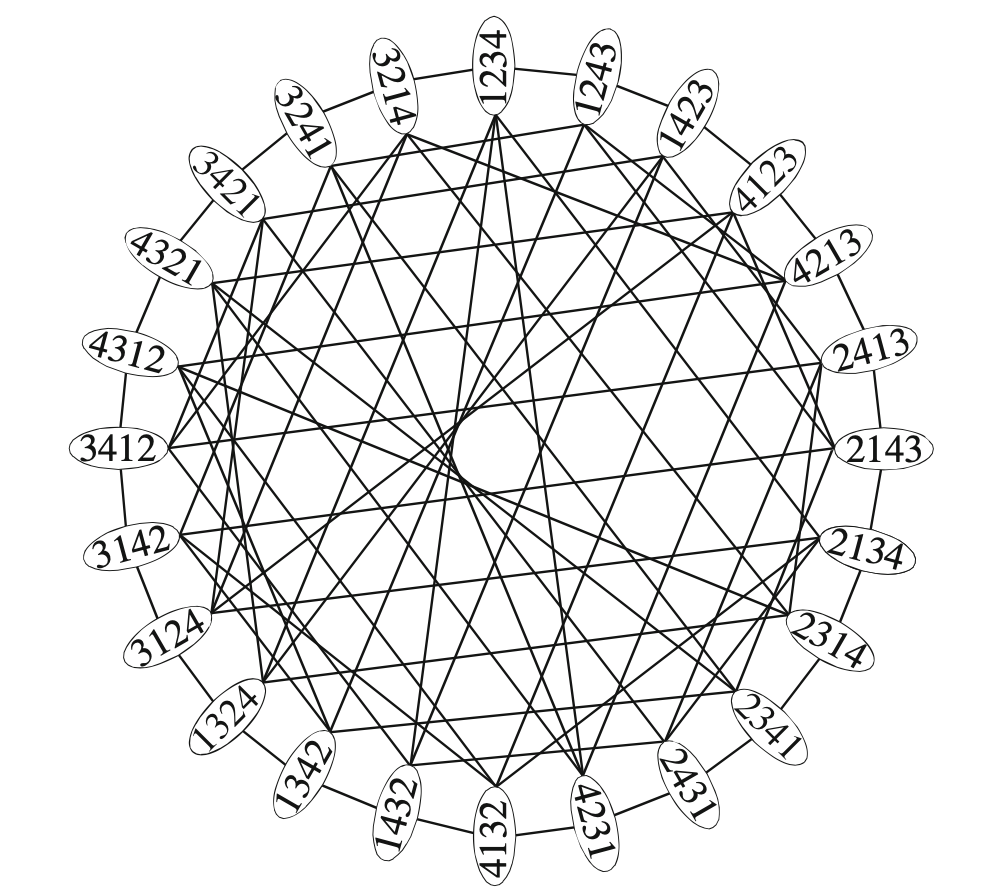
\includegraphics[width=0.74\textwidth]{assets/img/02_Grundlagen/Neighbourhood.png}
    }
    \caption{Nachbarschaftsbeziehungen einer Menge von Permutationen aus vier Elementen in Knotenform} 
    \label{img:example_neighbourhood}
    \source{\cite[][S. 57]{siarry_metaheuristics_2016} }
\end{figure}

Bei der Tabu-Suche stehen wie auch bei anderen Metaheuristiken, unterschiedliche Möglichkeiten zur Terminierung der Algorithmen zur Verfügung. Ein Algorithmus kann nach einer festen Anzahl an Iterationen oder CPU-Zeit beendet werden. Ein Algorithmus kann zudem auch nach einer bestimmten Anzahl an Iterationen, wo keine Verbesserung der Zielfunktion vorzufinden ist, terminiert werden. Eine weitere Möglichkeit ist, dass ein Algorithmus solange durchiteriert wird, bis ein definierter Schwellwert erreicht wurde. \cite[vgl.][S. 44]{gendreau_handbook_2019} 

\subsection{Simulated Annealing} \label{subsec:Grundlagen_SimulatedAnnealing}

Eine an der Physik, nämlich an der Metallurgie, orientierte Metaheuristik stellt \acf{SA} (dt. simuliertes Abkühlen) dar und wurde von den 3 IBM Wissenschaftlern Kirkpatrick, Gelatt und Vecchi im Jahre 1992 vorgeschlagen und im Jahr 1993 veröffentlicht. \cite[vgl.][S. 19]{siarry_metaheuristics_2016} \\

Für einen gegebenen Körper gilt es, nachdem dem Körper eine sehr hohe Temperatur zugeführt wurde, einen energetisch günstigen Zustand zu erreichen. Durch das Erhöhen der Temperatur zu einem sehr hohen Punkt wird die Struktur des Körpers zunächst geschmolzen. Der Körper befindet sich somit in einer flüssigen Phase, in welcher die Partikel des Körpers zufällig verteilt sind. Der Körper wird über das Abkühlen gemäß eines besonderen Temperaturschemas wieder in eine stabile Phase zurückgeführt und erreicht somit einen energetisch günstigen Zustand. Sowohl die initiale Temperatur als auch die Kühlungszeit müssen eine entsprechende Höhe aufweisen, da ansonsten ein metastabiler Zustand erreicht wird, in welcher die Energie nicht minimal ist. Der Prozess wird Härtung genannt, wenn die Temperaturabnahme nicht stetig ist und durch eine abrupte Abkühlung beeinflusst wird. Die Funktionsweisen und die Unterschiede zwischen dem Härtungs- und dem Abkühlungsprozess lassen sich über die Abbildung \ref{img:simulatedannealing_realworld} visualisieren. \cite[vgl.][S. 2 f.]{gendreau_handbook_2019} 

\begin{figure}[H]
    \centering
    \noindent\makebox[\textwidth]{%
    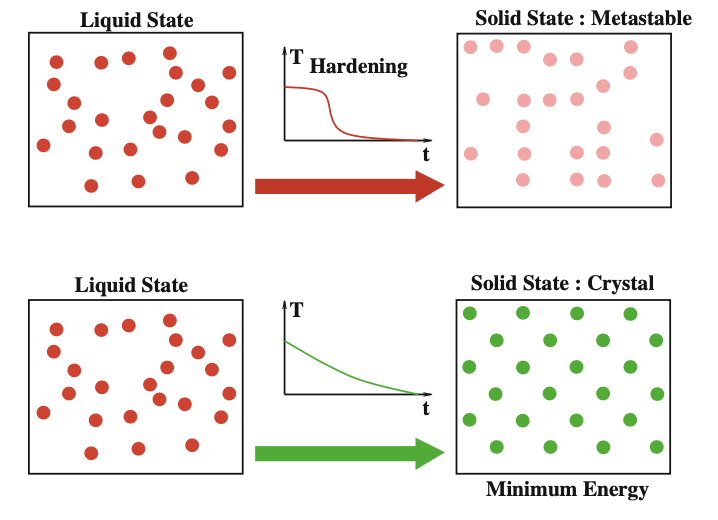
\includegraphics[width=0.48\textwidth]{assets/img/02_Grundlagen/SimulatedAnnealing_RealWorld.png}
    }
    \caption{Funktionsweise der Abkühlungs- und Härtungsprozesse} 
    \label{img:simulatedannealing_realworld}
    \source{\cite[][S. 3]{gendreau_handbook_2019} }
\end{figure}

Zwischen einem Optimierungsproblem und dem physikalischen System lassen sich Analogien ziehen. In der Physik wird die freie Energie betrachtet, bei dem Optimierungsproblem die Zielfunktion. Die Positionierung der Partikel stellt die Analogie zu den Parametern eines Problems dar. Das Ziel innerhalb eines physikalischen System liegt darin, dass ein energiearmer Zustand erreicht wird. Dies trifft ebenfalls bei Optimierungsproblemen zu, bei welchen Konfigurationen gesucht werden, welche als \glqq gut\grqq{} klassifiziert werden können oder im besten Fall am optimalsten sind. \cite[vgl.][S. 20]{siarry_metaheuristics_2016} 

\begin{lstlisting}[caption={Simulated Annealing (Quelle: \cite[vgl.][S. 714]{hosseinabadi_novel_2017}}), label=lst:simulatedannealing, mathescape=truexinputencoding={utf8}, extendedchars=false, escapeinside=``]
Create an initial solution $s$ inside the search space;
Select initial temperatur $T_0$;
Select rate of temperature decrease $\alpha \in [0.80, 0.99]$;
$T \leftarrow T_0$;  
while stopping criteria not satisfied do
    Select random solution $s' \in N(s)$;
    if f(s') < f(s)
        $s \leftarrow s'$;
    else
        $\Delta \leftarrow f(s') < f(s)$; 
        if random(0, 1) $< \exp(- \dfrac{\Delta}{T}$)
            $s \leftarrow s'$;
    $T \leftarrow T * \alpha$;
end
return the best solution;
\end{lstlisting}

Innerhalb des Algorithmus aus Listing \ref{lst:simulatedannealing} wird zunächst eine initiale Temperatur $T_0$ ausgewählt. Die Senkung anhand eines Temperaturschemas wird über eine Temperatursenkungsrate $\alpha \in [0.80, 0.99]$ realisiert. Wie auch bei der \ac{LS} wird eine initiale Lösung $s$ benötigt, welche zufällig oder über Heuristiken erzeugt werden können. Die initiale Lösung und Temperatur entsprechen dem flüssigen Zustand im Abkühlungsprozess. Nach jeder Iteration innerhalb des Algorithmus wird die Temperatur mit der Temperatursenkungsrate multipliziert $T \leftarrow T * \alpha$, was nach jeder Iteration zu einer Senkung der Temperatur führt. Um die Analogie zur Verfestigung zu realisieren, nutzt der Algorithmus die Nachbarschaftsfunktion, um so eine zufällige Lösung $s'$ auszuwählen. Über die Nutzung einer Akzeptanzfunktion gemäß Formel \ref{align:sa_acceptance} \cite[vgl.][S. 6]{gendreau_handbook_2019} und das Generieren einer zufälligen Zahl $r \in [0, 1]$ wird die Akzeptanz der Lösung $s'$ bestimmt. Sofern $r \leq P(s, s')$ gilt, wird die aktuelle Lösung überschrieben $s \leftarrow s'$. Das Annehmen von verschlechternden Lösungen im Algorithmus trägt maßgeblich zur Erkundung des Suchraums bei. Die Akzeptanz von schlechteren Lösungen sinkt über die Iterationen, da die ebenfalls sinkende Temperatur maßgebend zum Akzeptanzwert ist. Eine sinkende Temperatur impliziert, dass die Partikel innerhalb eines physikalischen Systems sich weniger stark bewegen. Gänzlich werden bei einer Temperatur $T \approx 0$ schlechtere Lösungen abgelehnt, was dazu führt, dass der Algorithmus lediglich als lokale Suche agiert. Es werden dann nur Lösungen angenommen, wenn die selektierte Lösung aus der Nachbarschaft besser als die aktuelle ist. \cite[vgl.][S. 5 f.]{gendreau_handbook_2019} \cite[vgl.][S. 21 f.]{siarry_metaheuristics_2016} 

\begin{align}
P(s, s') = \left\{\begin{array}{ll} 
        1 & \text{wenn $f(s') < f(s)$} \\
        e^{\Big(\dfrac{f(s) - f(s')}{T}\Big)} & \text{sonst} \\
     \end{array}\right. \label{align:sa_acceptance}
\end{align}

Wie bei der \ac{TS} stehen beim \ac{SA} unterschiedliche Stopkriterien zur Verfügung. Der Algorithmus von \cite[][S. 6 f.]{gendreau_handbook_2019} iteriert solange, bis die Temperatur bei $T \approx 0$ liegt. Der Algorithmus von \cite[][S. 714]{hosseinabadi_novel_2017} nutzt zusätzlich eine feste Anzahl an Iterationen, die durchlaufen werden müssen. Alternativ können die aus dem Abschnitt \ref{subsec:Grundlagen_TabuSearch} für die \ac{TS} vorgestellten Kriterien verwendet werden. Ein weitere Besonderheit stellt die Verwendung einer Boltzmann Konstante $k_B$ dar, welche zur Gewichtung der Temperatur in der Annahmefunktion beiträgt \cite[vgl.][S. 21]{siarry_metaheuristics_2016}. Durch die Verwendung einer Boltzmann Konstante $k_B$ lässt sich die Relevanz der Temperatur bei der Akzeptanzfunktion verändern.  

\input{pages/02_Grundlagen/023_EvolutionäreAlgorithmen}